\section{Supervised Classification}
A classification task aims at learning a function that assigns a label to a given input. Along with regression, classification is one of the  supervised learning tasks. One can find classification tasks in Computer Vision~\citep{lecun-mnisthandwrittendigit-2010,cifar-10,imagenet_cvpr09}, Natural Language Processing~\citep{vaswani2017attention}, Speech Recognition~\citep{dong2018speech}, etc. In this thesis, most examples will be from Computer Vision and Image Recognition. 
\subsection{Notations}
In this section, we formalize the task of classification. First, we define the notions of inputs and labels:
\begin{itemize}
    \item Consider an input space $\XX$, typically images. We assume this space is endowed with an arbitrary metric $d$, possibly a perception distance or any $\ell_p$ norm. In the following of the manuscript, unless it is specified, $(\XX,d)$ will be a \textit{proper} (i.e. closed balls are compact) \textit{Polish} (i.e. completely separable) metric space. Note that for any norm $\lVert\cdot\rVert$,  $(\mathbb{R}^d,\lVert\cdot\rVert)$ is a proper Polish metric space.
    \item Each input $x\in \XX$ has to be associated with a label $y$. A label is a descriptor of the input. The set of labels is discrete, and we designate it by $\YY:=\{1,\dots,K\}$. $\YY$ is endowed with the trivial metric  $d'(y,y') = \mathbf{1}_{y\neq y'}$. Note that $(\XX\times\YY,d\oplus d')$ is also a proper Polish space.
\end{itemize}

The purpose of classification is to learn a classifier $h:\XX\to\YY$. It is usual to learn a function $f:\XX\to\RR^K$ such that: $h(x) = \argmaxB_{k\in\YY}f_k(x)$. In a classification problem in machine learning, the data is assumed to be sampled from an unknown probability distribution $\PP$ over $\XX\times\YY$. We will assume from now that all the probability distributions we consider are Borel distributions. For any Polish Space $\mathcal{Z}$, we will denote $\mathcal{B}(\mathcal{Z})$ the Borel $\sigma$-algebra and the set of Borel distributions over $\mathcal{Z}$  will be denoted $\mathcal{M}_1^+(\mathcal{Z})$. We recall that on Polish space, all Borel probability distributions are Radon measures. We also recall the notion of \textit{universal measurability}: a set $A\subset \mathcal{Z}$ is said to be universally measurable if it is measurable for every \textit{complete} Borel probability measure. We also recall the notion of \emph{weak topology} on the space of probability distribution: we say that $\PP_n$ converges weakly towards $\PP$ if for every bounded continuous function $f$, $\int fd\PP_n\to\int f d\PP$. Note that calling this property weak topology is an abuse of language, it is closer to a notion of weak-$\star$ topology. 

When $\ZZ$ and $\ZZ'$ are two measurable spaces endowed with their Borel $\sigma$-algebra (unless specified), we will denote $\mathcal{F}(\ZZ,\ZZ')$ the space of measurable functions from $\ZZ$ to $\ZZ'$. Without loss of generality, when $\ZZ'=\RR$, we will simply denote: $\mathcal{F}(\ZZ):=\mathcal{F}(\ZZ,\ZZ')$.




\subsection{Classification Task in Supervised Learning}


In standard classification, we usually aim at maximizing the accuracy of the classifier, or equivalently, at minimizing the risk associated with the $0/1$ loss defined as follows.

    
\begin{definition} Let $\PP$ be a Borel probability distribution over $\XX\times\YY$. Let $h:\XX\to\YY$ be a Borel measurable classifier. Then, the risk of $h$ associated with $0/1$ loss (or error of $h$) is defined as:
\begin{align}
   \risk_{\PP}(h):=\PP(h(x)\neq y) = \EE_{(x,y)\sim\PP}\left[\mathbf{1}_{h(x)\neq y}\right]
\end{align}
The Optimal Bayes risk is defined as the optimal risk over measurable classifiers $\mathcal{F}(\XX,\YY)$:
\begin{align}
    \risk^\star_{\PP}:=\inf_{h\in\mathcal{F}(\XX,\YY)}\risk_{\PP}(h)
 \end{align}
If $f:\XX\to\RR^K$, then the risk of $f$ is defined as $\risk_{\PP}(f):=\PP(\argmaxB_{k\in\YY}f_k(x)\neq y)$
\end{definition}
Note that this quantity is well-defined when $h$ or $f$ is Borel or universally measurable. The optimal classifier is called the \emph{Optimal Bayes  classifier} and is defined as $h^\star(x) = \argmaxB_k\PP(y=k\mid x)$. We remark that the disintegration theorem ensures that $x\mapsto \PP(y=k\mid x)$ is indeed Borel measurable. 

In practice, the access to the Optimal Bayes  classifier is not possible because it requires full knowledge of the probability distribution $\PP$ which is not the case in general. Instead, in the supervised learning setting, the learner has access to data points $\{(x_1,y_1),\dots,(x_\numsamples,y_\numsamples)\}$, that constitutes the \emph{training set}. Knowing the Optimal Bayes classifier on training points is not sufficient to generalize on points out of the training set. Hence, one needs to reduce the search space of measurable functions to a much smaller one, denoted $\mathcal{H}$ in the sequel. The $0/1$ loss is not convex neither continuous, and minimizing directly the 0/1 loss risk  on $\mathcal{H}$ might be NP-hard even for simple set of hypotheses as linear classifiers. We usually minimize a well-chosen surrogate loss function $\loss$. A \textit{loss function} $\loss:\mathbb{R}^K\times\YY\to\mathbb{R}$ is a non-negative Borel measurable function. An example of such a loss is the cross entropy loss defined as $\loss(f(x),y)=-\sum_{i=1}^K \mathbf{1}_{y=i}\log f_i(x)$
where $f_i(x)$ is the probability learned by the model with input $x$ belonging to the class $i$. Hence, the objective is to minimize the empirical risk associated with $\mathcal{H}$ using the loss $\loss$  defined as:
\begin{align*}
\riskemp_{\loss}(f):= \frac{1}{\numsamples}\sum_{i=1}^\numsamples \loss(f(x_i),y_i).
\end{align*}
% In the next sections~\ref{xxx} and~\ref{xxx}, we recall the main results about surrogate losses for the $0/1$ loss and generalization properties of the classifiers.



% \paragraph{Usual Datasets in Image Classification}
% %Images are embeddings in pixels laying in $[0,255]$ and then normalized to $[0,1]$. These images can be black and white, hence encoded on only one channel, or colorful and then encoded on three channels, often, Red, Green, Blue (RGB). The images are of diverse qualities, the number of pixels quantifies this quality.  
% In this PhD thesis, although the results are general and applicable to every type of data, we mainly focus on image classification tasks. Three datasets are mainly used in image classification:
% \begin{itemize}
%     \item \textbf{MNIST~\citep{lecun1998mnist}:} A dataset of black and white low-quality images representing the $10$ digits. The training set contains $50000$ images and test set $10000$ images. These images are of dimension $28\times28\times 1$ ($784$ in total). This dataset is known to be easy ($>99\%$ can be obtained using simple classifiers). 
%     \item \textbf{CIFAR10 and CIFAR100~\citep{krizhevsky2009learning}:} Datasets of colored low-quality images representing the $10$ labels and $100$ labels for respectively CIFAR10 and CIFAR100. Each training set contains $50000$ images and test set $10000$ images. These images are of dimension $32\times32\times 3$ ($3072$ in total). The current state-of-the-art on CIFAR10 in standard classification is $>99\%$ of accuracy, but asks advanced methods to reach such a score. On CIFAR100, the current state-of-the-art is around $94\%$. 
%     \item \textbf{ImageNet~\citep{imagenet_cvpr09}:} ImageNet refers to a dataset containing $1.2$ million of images labeled into $1000$ classes. Images are of diverse qualities, but models often takes input of dimension $224\times224\times 3$ (dimension $150528$ in total). The current state-of-the-art on ImageNet is about $87\%$. Further than the standard dataset, ImageNet project is still in development: the project gathers $14197122$ images and $21841$ labels on August 31th, 2021.   




% \end{itemize}


\paragraph{Neural Networks} A popular set of classifiers are Neural Networks. They gained in popularity due to their exceptional performances in Image Recognition~\citep{krizhevsky2012imagenet,he2016deep} or Natural Language Processing for instance~\citep{vaswani2017attention}. In its simpler form, a neural network is a concatenation of linear operators and non-linear functions (called \emph{activations}). This concatenation are called \emph{layers}. Formally a neural network with $L$ layers writes:
\begin{align*}
    f(x) = \left(W_L\sigma\left(W_{L-1}\dots \sigma\left(A_1x+b_1\right)\dots\right)+b_L\right)
\end{align*}
where $W_i$ are called the weight matrices and $b_i$ the biases. In the case of image recognition, the weights may have a special structure of convolution: such networks are called \emph{Convolutional Networks}. We illustrate a convolutional layer in Figure~\ref{fig:convnet}.

\begin{figure}
    \centering
    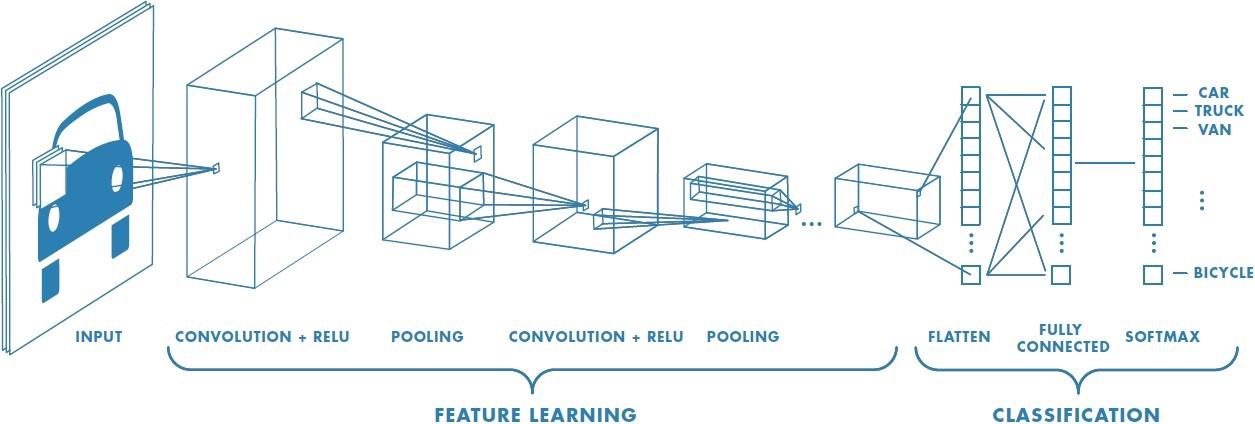
\includegraphics[width=0.9\textwidth]{Images/conv_net.jpeg}
    \caption{Illustration of a convolutional neural network: stacking convolutional operators and non-linear activation functions.}
    \label{fig:convnet}
\end{figure}

To train neural networks, the backpropagation is a standard algorithm based on the chain rule. This algorithm is subject to gradient vanishing, or gradient explosion issues. To circumvent these problems, many tricks were proposed as  using ReLU-like activation functions~\citep{xu2015empirical,ramachandran2017searching}, Dropout~\citep{srivastava2014dropout}, Batch Normalization~\citep{ioffe2015batch} or the use of Residual Layers~\citep{he2016deep}. More, despite their popularity, it is difficult to understand the outstanding performances of neural networks.



\subsection{Surrogate losses, consistency and calibration} 

\paragraph{Binary Classification.} In this section, we recall the main results about surrogate losses in binary classification. We assume that $\YY = \{-1,+1\}$. In this case, a classifier is a measurable function $f:\XX\to\RR$ such that an input $x$ is classified as $1$ if $f(x)>0$ and as $-1$ if $f(x)\leq 0$. Then the $0/1$ loss is defined as $\mathbf{1}_{y\times sign(f(x))\leq0}$. As mentioned earlier, optimizing the risk associated with the $0/1$ loss is a difficult task. We need to properly introduce notions of surrogate losses. 

A margin loss is a loss $\loss$ such that there exist a measurable function $\phi:\RR\to\RR_+$, satisfying, $\loss(x,y,f) =\phi(yf(x))$. The risk associated with a margin loss $\phi$ is then $\risk_{\phi,\PP}(f):=\mathbb{E}_\PP\left[\phi(yf(x))\right]$. A loss $\phi$ is said to be \emph{classification-consistent} if every minimizing sequence for the risk associated with the $\phi$ loss is also a minimizing sequence for the risk associated with the $0/1$-loss. In other words, for a given $\PP\in\mathcal{M}_1^+(\XX\times\YY)$, $\phi$ is classification-consistent for $\PP$ if for all sequences $(f_n)_{n\in\mathbb{N}}$ of measurable functions:
\begin{align}
    \mathcal{R}_{\phi,\PP}(f_n)\to \mathcal{R}_{\phi,\PP}^\star:=\inf_{f\in\mathcal{F}(\XX)}\mathcal{R}_{\phi,\PP}(f)\implies\mathcal{R}_{\PP}(f_n)\to \mathcal{R}_{\PP}^\star
\end{align}

 While this notion seems complicated to study,~\cite{zhang2004statistical,bartlett2006convexity,steinwart2007compare} have focused on a relaxation named \emph{calibration}. A loss is said to be \emph{classification-calibrated} if for every $\varepsilon>0$, there exists $\delta>0$ such that for every $\alpha\in\RR$ and $\eta\in[0,1]$:
\begin{align*}
    \eta\phi(\alpha)+(1-\eta)\phi(-\alpha)-\min_{\beta\in\RR}\left[ \eta\phi(\beta)+(1-\eta)\phi(-\beta)\right]\leq \delta\implies sign\left((\eta-\frac12)\alpha\right)=1
\end{align*}
We remark the notion of calibration is basically a pointwise notion of consistency with $\eta$ corresponding to $\PP(y=1|x)$.~\citet{zhang2004statistical,bartlett2006convexity,steinwart2007compare} proved the equivalence of the two notions in the case of standard-binary classification. In particular, they show that a wide range of convex margin losses are actually classification-consistent: if $\phi$ is convex and differentiable at $0$, then $\phi$ is calibrated if and only if $\phi'(0)<0$.


The problem of consistency have been investigated in the case of multi-label classification by~\citet{zhang2004multi}. The results can be similarly derived, and it was show that large range of convex functions are actually consistent for classification problems.

% We say that a loss $L_2$ is said to be consistent with respect to a loss $L_1$ if consistency holds for every distribution $\PP$. 

% \begin{definition}[Loss function] A loss function is a function $\loss:\XX\times\YY\times \mathcal{F}(\XX)\to \mathbb{R}$ such that $\loss(\cdot,\cdot,f)$ is a Borel measurable for all $f\in\mathcal{F}(\XX)$. 
% \end{definition}


% Similarly to risk associated with the $0/1$ loss, 
% \begin{definition}[$\loss$-risk of a classifier]
% For a given measurable loss $\loss$, and a Borel probability distribution $\PP$ over $\XX\times\YY$ we define the risk of classifier $f$ associated with the loss $\loss$ and a distribution $\PP$ as:
% \begin{align*}
%      \mathcal{R}_{\loss,\PP}(f) := \mathbb{E}_{(x,y)\sim\PP}\left[\loss(x,y,f)\right].
% \end{align*}
% We also define the optimal risk associated with the loss $\loss$:
% \begin{align*}
%          \mathcal{R}_{\loss,\PP}^\star := \inf_{f\in\mathcal{F}(\XX)}\mathcal{R}_{\loss,\PP}(f)
% \end{align*}
% \end{definition}


% The risk of a classifier is then defined as the average loss over the distribution $\PP$. The loss $L$ is difficult to optimize in practice: the loss might, for instance, not convex  not differentiable or continuous. It is then often preferred to optimize a surrogate loss function instead. In the literature~\citep{zhang2004statistical,bartlett2006convexity,steinwart2007compare}, the notion of surrogate losses has been studied as a consistency problem: a surrogate loss is said to be consistent if any minimizing sequence of classifiers for the  risk associated with the surrogate loss is also one for the risk associated with $L$. Formally, the notion of consistency as  follows.

% \begin{definition}[Consistency]
% Let $L_1$ and $L_2$ be two loss functions. For a given $\PP\in\mathcal{M}_1^+(\XX\times\YY)$, $L_2$ is said to be consistent for $\PP$ with respect to $L_1$ if for all sequences $(f_n)_n \in \mathcal{F}(\XX)^\mathbb{N}$ :
% \begin{align}
%     \mathcal{R}_{L_2,\PP}(f_n)\to \mathcal{R}_{L_2,\PP}^\star\implies\mathcal{R}_{L_1,\PP}(f_n)\to \mathcal{R}_{L_1,\PP}^\star
% \end{align}
% We say that a loss $L_2$ is said to be consistent with respect to a loss $L_1$ if consistency holds for every distribution $\PP$.
% \end{definition}

\subsection{Empirical Risk Minimization and Generalization}
\label{sec:erm-results}
As mentioned earlier, the learner has access to training points  $\{(x_1,y_1),\dots,(x_\numsamples,y_\numsamples)\}$ and not to the whole distribution. We aim at learning the classifier on a set of functions $\mathcal{H}$. The classifier $\hat{f}_\numsamples $ is then chosen to minimize the empirical risk given a loss $\loss$:
\begin{align*}
    \hat{f}_\numsamples = \argminB_{f\in\mathcal{H}}\riskemp_{\loss}(f)= \argminB_{f\in\mathcal{H}}\frac{1}{\numsamples}\sum_{i=1}^\numsamples \loss(f(x_i),y_i).
\end{align*}

Since the learning procedure takes into account a finite number of samples and a set $\mathcal{H}$ of hypotheses, one need to control the risk of the classifier $\hat{f}_\numsamples$.

\paragraph*{Risk Decomposition and bias-complexity tradeoff.} The excess risk of a classifier is defined as the difference between the risk and the optimal risk: $\risk_\loss(f_n) - \risk_\loss^\star$. The excess risk can be decomposed as follows:
\begin{align*}
    \risk_\loss( \hat{f}_\numsamples) - \risk_\loss^\star = \left(\risk_\loss( \hat{f}_\numsamples) - \risk_{\loss,\mathcal{H}}^\star\right)+ \left(\risk_{\loss,\mathcal{H}}^\star - \risk_\loss^\star\right)
\end{align*}

with $\risk_{\loss,\mathcal{H}}^\star = \inf_{f\in\mathcal{H}}\risk_\loss(f)$. The two terms in the previous decomposition corresponds respectively to:
\begin{itemize}
    \item \textbf{The estimation risk}:  the empirical risk $\risk(\hat{f}_\numsamples)$ (i.e., training error) is only an estimate of the optimal risk, and so $\hat{f}_\numsamples$   is only an estimate of the predictor minimizing the true risk. The estimation risk depends on the training set size $\numsamples$ and on the size, or complexity, of  $\mathcal{H}$.  The more samples we have the smaller will be the estimation risk and more complex $\mathcal{H}$ is the larger the estimation error will be.
    \item \textbf{The approximation risk}: the approximation risk is the error made by optimizing over $\mathcal{H}$ instead of minimization over the whole space of measurable functions. As  the function space $\mathcal{H}$ grows, the approximation naturally decreases. 
\end{itemize}

This decomposition induces a tradeoff on the complexity of $\mathcal{H}$ named \emph{bias-complexity tradeoff} or \emph{bias-variance tradeoff}. On one hand, if $\mathcal{H}$ is not enough rich, then the estimation risk would be small, but the approximation error can be large, it is called \emph{underfitting}. On the other hand, if $\mathcal{H}$ is too rich, then the approximation risk would be small but the estimation error large, it is called \emph{overfitting}. To overcome these issues in practice, it is usual to add a regularization parameter to the empirical risk depending on the set $\mathcal{H}$:
\begin{align*}
    \hat{f}_\numsamples = \argminB_{f\in\mathcal{H}}\riskemp_{\loss}(f) +\lambda\times\Omega_\mathcal{H}(f)= \argminB_{f\in\mathcal{H}}\frac{1}{\numsamples}\sum_{i=1}^\numsamples \loss(f(x_i),y_i)+\lambda\times\Omega_\mathcal{H}(f).
\end{align*}

The convergence of regularized least squares regression has been largely studied on Reproducing Kernel Hilbert Space (RKHS). A RKHS $(\mathcal{H},\langle\cdot,\cdot\rangle_\mathcal{H})$ is characterized by a symmetric, positive definite function called a kernel over $\XX$ such that for all $f\in\mathcal{H}$ and $x\in\XX$, $f(x)= \langle f,k(x,\cdot)\rangle_\mathcal{H}$. In this case, the regularization parameter $\Omega_\mathcal{H}(f)$ is the square norm of $f$: $\lVert f\rVert_\mathcal{H}^2$. 


\paragraph{Uniform Convergence.} Since $\hat{f}_\numsamples$ is dependent on the training samples, it is usually difficult to estimate $\risk(\hat{f}_\numsamples)$ from training samples. A natural thing to do is to upperbound this quantity using:
\begin{align*}
    \lvert\riskemp(\hat{f}_\numsamples) - \risk(\hat{f}_\numsamples)\rvert\leq\sup_{f\in\mathcal{H}}    \lvert\riskemp(f) - \risk(f)\rvert
\end{align*}

The convergence of the right-end term is referred as uniform convergence or Provably Approximately correct (PAC) learning~\citep{valiant1984theory}. It can be bounded either with high probability or in expectation (i.e. $L^1$ convergence). We remark the speed of convergence depends on the complexity of $\mathcal{H}$: more complex $\mathcal{H}$ is, the slower the convergence will be, hence exhibiting again a tradeoff on the expressivity of $\mathcal{H}$. There have been a  lot of research that proposed tools to study this convergence. Now, we recall a fundamental tool, namely the Rademacher complexity.


The Rademacher complexity was introduced by~\cite{bartlett2002rademacher} to study the problem of uniform convergence. Given a set of functions~$\mathcal{H}$, and a set of observations $S=\{z_1,\dots,z_\numsamples\}$ from a distribution $\PP$, the empirical Rademacher complexity is defined as:
\begin{align*}
    \widehat{\text{Rad}}_S(\mathcal{H}):=\frac2\numsamples\mathbb{E}_{\sigma}\left[\sup_{h\in\mathcal{H}}\lvert\sum_{i=1}^\numsamples\sigma_i h(z_i)\rvert\right]
\end{align*}
where $\sigma_i$ are independent samples from Rademacher law: $P[\sigma_i =+1] = P[\sigma_i =-1]=\frac12$. The Rademacher complexity satisfy the following composition property of Rademacher complexity: when $\phi$ is a $M$-Lipschitz function:
\begin{align*}
    \widehat{\text{Rad}}_S(\phi\circ\mathcal{H}) \leq M\widehat{\text{Rad}}_S(\mathcal{H})
\end{align*}
This property is particularly useful because it allows to study the Rademacher complexity regardless the loss function.
When $\mathcal{H}$ is not too complex (for instance, finite set or linear classifiers), one can bound the Rademacher complexity  by $O(n^{-1/2})$. It was proven by~\citet{bartlett2002rademacher} that the Rademacher complexity upperbounds the uniform risk error as follows:
\begin{align*}
    \mathbb{E}_{S\sim\PP^\numsamples}\left[\sup_{h\in\mathcal{H}}\lvert e_S(h)-e_\PP(h)\rvert\right]\leq 2\mathbb{E}_{S\sim\PP^\numsamples}\left[\widehat{\text{Rad}}_S(\mathcal{H})\right]
\end{align*}
where $e_\PP(h)=\mathbb{E}_{z\sim\PP}\left[h(z)\right]$ and $e_S(h)=\frac1\numsamples \sum_{i=1}^\numsamples h(z_i)$. This property leads to the following generalization error bound derived from classical concentration bounds: with probability $1-\delta$ (over the sampling $S$), for every $h\in \mathcal{H}$:
\begin{align*}
    e_S(h)-e_\PP(h)\leq 2  \widehat{\text{Rad}}_S(\mathcal{H})+4\sqrt{\frac{2\log(4/\delta)}{n}}\quad.
\end{align*}


Rademacher complexity along with VC-dimension~\citep{vapnik1998} are the main tools for deriving generalization bounds. The two concepts are linked and one can upperbound the Rademacher complexity with the VC dimension.



